% --------------------------------------------------------------
% This is all preamble stuff that you don't have to worry about.
% Head down to where it says "Start here"
% --------------------------------------------------------------
 

% --------------------------------------------------------------
%                         Start here
% --------------------------------------------------------------
 
%\renewcommand{\qedsymbol}{\filledbox}

\title{TUTORIAL 4}%replace X with the appropriate number
\author{TRISTAN GLATARD\\ %replace with your name
COMP 361 Numerial Methods} %if necessary, replace with your course title
\date{October 5, 2018} 
\maketitle

\begin{exercise}{1} %You can use theorem, proposition, exercise, or reflection here. 
Draw a plot of $f(x) = cosh(x)cos(x)-1$ in the range $0 \leq x \leq 10$. (a) Verify from the
plot that the smallest positive, nonzero root of $f(x)=0$ lies in the interval (4, 5).
(b) Show graphically that the Newton-Raphson formula would not converge to
this root if it is started with $x = 4$.

\textbf{Solution.} 

Plot of the function is done with Google's help. \textit{Hint: just type the function in Google, it will draw the plot.}

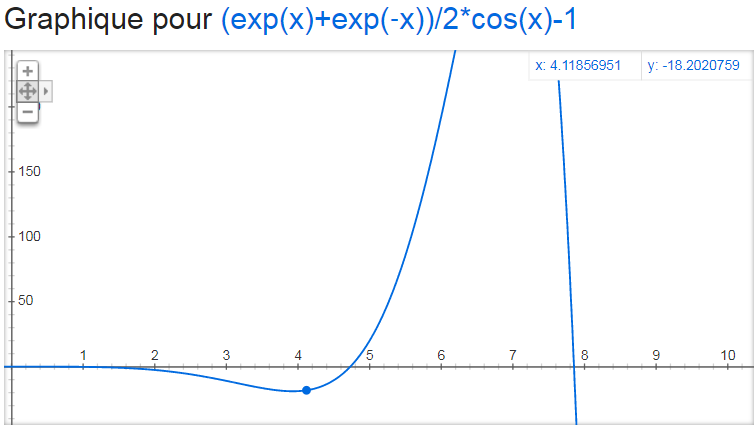
\includegraphics[]{coshxcosx-1.png}

In this plot, we can see that if we start Newton-Raphson method with x=4, the approximation will be out of range [4,5] ($\approx  10.66$, try to verify this!). This is because the approximation is calculated by the tangent line which is not sloppy at $x=4$. (Try to verify this! Hint: the slope of the tangent line at $x_0$ is  $f^\prime(x_0)$. Compare $f^\prime(4)$ and $f^\prime(5)$ )

\end{exercise}

%EXERCISE 2-----------------------------------------------------
\begin{exercise}{2} %You can use theorem, proposition, exercise, or reflection here.  
A zero $x = r$ of $P_n(x)$ is given. Verify that r is indeed a zero, and then deflate the polynomial; that is, find $P_{n-1}(x)$ so that $P_n(x) = (x-r)P_{n-1}(x)$.
\begin{align}
1. P_3(x) &= 3x^3 + 7x^2 - 36x + 20, r = -5 \notag \\
2. P_4(x) &= x^4 - 3x^2 + 3x - 1, r = 1 \notag
\end{align}

\textbf{Solution.}

1. First, verify r = -5 is indeed a zero
\begin{align}
P_3(-5) &= 3*(-5)^3 + 7*(-5)^2 - 36*(-5) + 20 \notag \\
&=-3*125 + 7*25 + 180 + 20 = 0 \notag 
\end{align}

The coefficients of $P_3(x)$ are:
\begin{align}
a_3 = 3, a_2 = 7, a_1 = -36, a_0 = 20 \notag 
\end{align}

Now the deflation of $P_3(x)$ is done as: 
\begin{align}
b_2 &= a_3 = 3 \notag \\ 
b_1 &= a_2 + rb_2 = 7 + (-5)*3 = -8 \notag \\
b_0 &= a_1 + rb_1 = -36 + (-5)(-8) = 4 \notag 
\end{align}

And the deflated polynomial is
\begin{align}
P_2(x) &= 3x^2 - 8x + 4 \notag 
\end{align}

2. First, verify r = 1 is indeed a zero
\begin{align}
P_4(1) &= (1)^4 - 3*1^2 + 3* 1 - 1 \notag \\
&= 0 \notag
\end{align}

The coefficients of $P_4(x)$ are:
\begin{align}
a_4 = 1, a_3 = 0, a_2 = -3, a_1 = 3, a_0 = -1 \notag 
\end{align}

Now the deflation of $P_4(x)$ is done as: 
\begin{align}
b_3 &= a_4 = 1 \notag \\ 
b_2 &= a_3 + rb_3 = 0 + 1*1 = 1 \notag \\ 
b_1 &= a_2 + rb_2 = -3 + 1*1 = -2 \notag \\
b_0 &= a_1 + rb_1 = 3 + 1*(-2) = 1 \notag
\end{align}


And the deflated polynomial is
\begin{align}
P_3(x) &= x^3 + x^2 - 2x + 1 \notag 
\end{align}
\end{exercise}


%EXERCISE 2-----------------------------------------------------
\begin{exercise}{3} %You can use theorem, proposition, exercise, or reflection here.  
A zero $x = r$ of $P_n(x)$ is given.Determine all the other zeros of $P_n(x)$ by
using a calculator. You should need no tools other than deflation and the quadratic
formula.
\begin{align}
1. P_3(x) &= x^3+1.8x^2-9.01x-13.398, r =-3.3\\
2. P_3(x) &= x^3-6.64x^2+16.84x-8.32, r = 0.64
\end{align}

\textbf{Solution.} 

\textbf{Reminder}: the quadratic equation of the form $ax^2 + bx +c = 0$ has two roots:
\begin{align}
x_{1,2} = \frac{-b \pm \sqrt[]{\Delta}}{2a}
\end{align}

where $\Delta = b^2 - 4ac$ 

1. The coefficients of $P_3(x)$ are:
\begin{align}
a_3 = 1, a_2 = 1.8, a_1 = -9.01, a_0 = -13.398 \notag 
\end{align}

Now the deflation of $P_3(x)$ is done as: 
\begin{align}
b_2 &= a_3 = 1 \notag \\ 
b_1 &= a_2 + rb_2 = 1.8 + (-3.3)*1 = -1.5 \notag \\
b_0 &= a_1 + rb_1 = -9.01 + (-3.3)(-1.5) = -4.06 \notag 
\end{align}

And the deflated polynomial is
\begin{align}
P_2(x) &= x^2 - 1.5x - 4.06 \notag 
\end{align}


The above quadratic has two roots, as shown in (3): 
\begin{align}
x_{1,2} &= \frac{1.5 \pm \sqrt[]{1.5^2+4*4.06}}{2} \notag \\
x_1 &= -1.4 \notag \\
x_2 &= 2.9 \notag
\end{align}

2. The coefficients of $P_3(x)$ are:
\begin{align}
a_3 = 1, a_2 = -6.64, a_1 = 16.84, a_0 = -8.32 \notag 
\end{align}


Now the deflation of $P_3(x)$ is done as: 
\begin{align}
b_2 &= a_3 = 1 \notag \\ 
b_1 &= a_2 + rb_2 = -6.64 + 0.64*1 = -6 \notag \\
b_0 &= a_1 + rb_1 = 16.84 + 0.64*(-6) = 13 \notag 
\end{align}


And the deflated polynomial is
\begin{align}
P_2(x) &= x^2 - 6x + 13 \notag 
\end{align}



The above quadratic has two roots as shown in (3): 
\begin{align}
x_{1,2} &= \frac{6 \pm \sqrt[]{6^2-4*13}}{2} \notag \\
&=3 \pm \sqrt[]{-4} \notag \\
&= 3 \pm 2i \notag \\
x_1 &= 3 + 2i \notag \\
x_2 &= 3 - 2i \notag
\end{align}
\end{exercise}
% --------------------------------------------------------------
%     You don't have to mess with anything below this line.
% --------------------------------------------------------------
 
\end{document}
